
\chapter{Technical choice}
\label{chap:choice}

\section{Application created for test}

As it was explain before, I have to protect specific applications. To do my tests, and prove the concept of my
work, I choose to create a simple application. I plan to add some security issue to be more realistic.~\\


This application has three states, and two parts. Firstly, there is an admin interface which contains the state
admin. This interface is connected on the port 9000. Only one specific known computer can access to this interface.
Of course, the aim of attackers is to arrive in this state.

Then there is the main application. It is connected to the port 9124, and everybody can connect to it. There is two
states ping and pong. If the application is in the state ping and the user send <<topong>> the application go to
state pong, and if the application is in the state pong and the user send <<toping>> the application go to the
state ping. There is also an unknown backdoor, if the user is in the state ping for the third time and he send
<<admin>>, the application go to the admin interface.

The figure \ref{fig:appli} represent a model of our application.


\begin{figure}[!h]
  \centering
  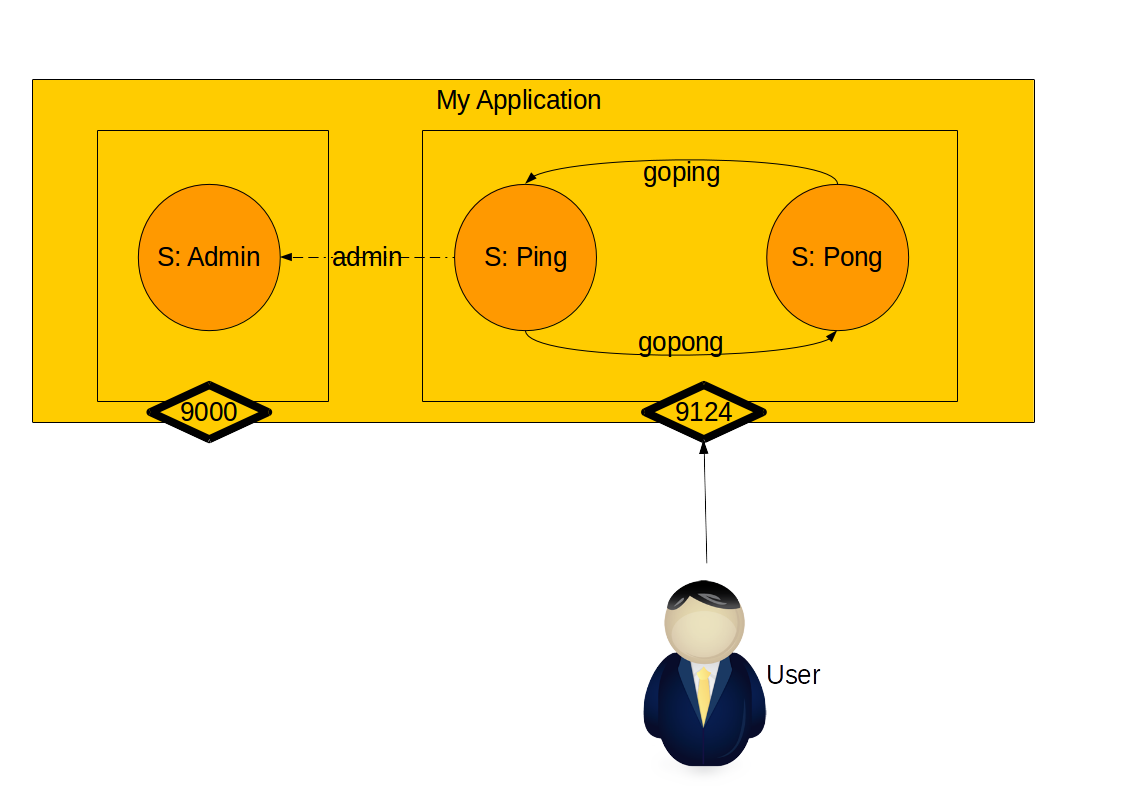
\includegraphics[width=0.9\textwidth]{appli}
  \caption{Model of the application}
  \label{fig:appli}
\end{figure}

\section{IDS}

To monitor the network between my applications, I have to install an IDS. In this project, my IDS only need to check
network packets and send alert when it detects some pattern. So I choose to use an IDS which use a misuse detection.

Moreover, my IDS only need to raise alert and save them. It is possible to find on the market of open source
software many IDS which do that. So I choose one of the most popular open source IDS, SELKS.

\section{SIEM}

Then, for the SIEM I had to made a choice: use an open source solution of SIEM, or implement my own solution. The
table \ref{tab:preludevssiem} lists advantages and drawback of the two solutions.

\begin{table}[h]
  \centering
  \begin{tabularx}{1.0\linewidth}[h]{|X|X|}
    \hline
    \multicolumn{2}{|>{\centering\hsize=2\hsize}X|}{\textbf{Prelude}}\\
    \hline
    Advantages & Drawbacks \\
    \hline
    Already implemented & Need to connect it to SELKS \\
    \hline
    More modular  & Not adapted to my problem \\
    \hline
               & Need to configure it \\
    \hline
               & Heavy solution \\


    %%%%%%%%%%%%%%%%%%%%%%%%%%%%%%%%%%%%%%%%
    \hline
    \hline
    \multicolumn{2}{|>{\centering\hsize=2\hsize}X|}{\textbf{My SIEM}}\\
    \hline
    Advantages & Drawbacks \\
    \hline
    Well adapted for my problem & Need time to implement it \\
    \hline
    Less heavy & Only adapted for my problem\\

    \hline

  \end{tabularx}
  \caption{Prelude vs my SIEM}
  \label{tab:preludevssiem}
\end{table}

For all the reasons cited on the previous table, I choose to implement my own SIEM.


%%% Local Variables:
%%% mode: latex
%%% TeX-master: "../rapport_de_base"
%%% End:
